\documentclass{article}
\usepackage{ctex}
\usepackage{graphicx}
\usepackage{amsmath}
\usepackage{indentfirst}
\usepackage{titlesec}
\usepackage{setspace}
\usepackage{subfigure}
\usepackage{caption}
\usepackage{float}
\usepackage{booktabs}
\usepackage{geometry}
\usepackage{multirow}
\geometry{left=1.2cm,right=1.2cm,top=2cm,bottom=2cm}
\title{\songti \zihao{2}\bfseries HW3第6题舍选法Gauss-Lorentz报告}
\titleformat*{\section}{\songti\zihao{4}\bfseries}
\titleformat*{\subsection}{\songti\zihao{5}\bfseries}
\renewcommand\thesection{\arabic{section}}
\author{王启骅 PB20020580}
\begin{document}
	\maketitle
	\section{题目}
对两个函数线型(Gauss 分布和 类Lorentz 型分布),设其一为 p(x),另一为
F(x),其中常数$ a\neq b\neq 1 $ , 用舍选法对 p(x) 抽样。将计算得到的归一化频数分布直方图
与理论曲线 p(x) 进行比较,讨论差异,讨论抽样效率。


其中$ Gauss\sim \ exp(-ax^2) $ , $ Loretz \sim \ \frac{1}{1+bx^4} $
	\section{算法原理}
根据计算分析得取a=3,b=2,c=1.5可以使$  c/(1+bx^4)\ge \sqrt{\frac{a}{\pi}}exp(-ax^2) $在实轴上全部成立,其中$ \sqrt{\frac{a}{\pi}} $为归一化因子,并令
\begin{equation}
	F(x)=\frac{c}{1+bx^4}
\end{equation}
\begin{equation}
	p(x)=\sqrt{\frac{a}{\pi}}\exp(-ax^2)
\end{equation}


产生在[0,1]均匀分布的随机数列$ \xi_1,\xi_2 $


\begin{equation}
	\xi_1=\frac{\int_{-\infty}^{\xi_x}F(x)dx}{\int_{-\infty}^{+\infty}F(x)dx}=
	\frac{\ln(\frac{\sqrt{2}\xi_x^2+2^{0.75}\xi_x+1}{\sqrt{2}\xi_x^2-2^{0.75}\xi_x+1})+2\arctan(2^{0.75}\xi_x+1)-2\arctan(1-2^{0.75}\xi_x)}{4\pi}+0.5
\end{equation}
\begin{equation}
	\xi_y=\xi_2F(\xi_x)=\frac{1.5\xi_2}{1+2\xi_x^4}
\end{equation}


使用二分法解方程(3)即可得到$ \xi_x(\xi_1) $,并判断条件$ \xi_y<p(\xi_x) $,则取$ x=\xi_x $,否则舍去该点。之后将点数据x输入到txt文件,并用python读取统计画图。


	
	\section{结果}
	
	\begin{figure}[!h]
		
		\centering
		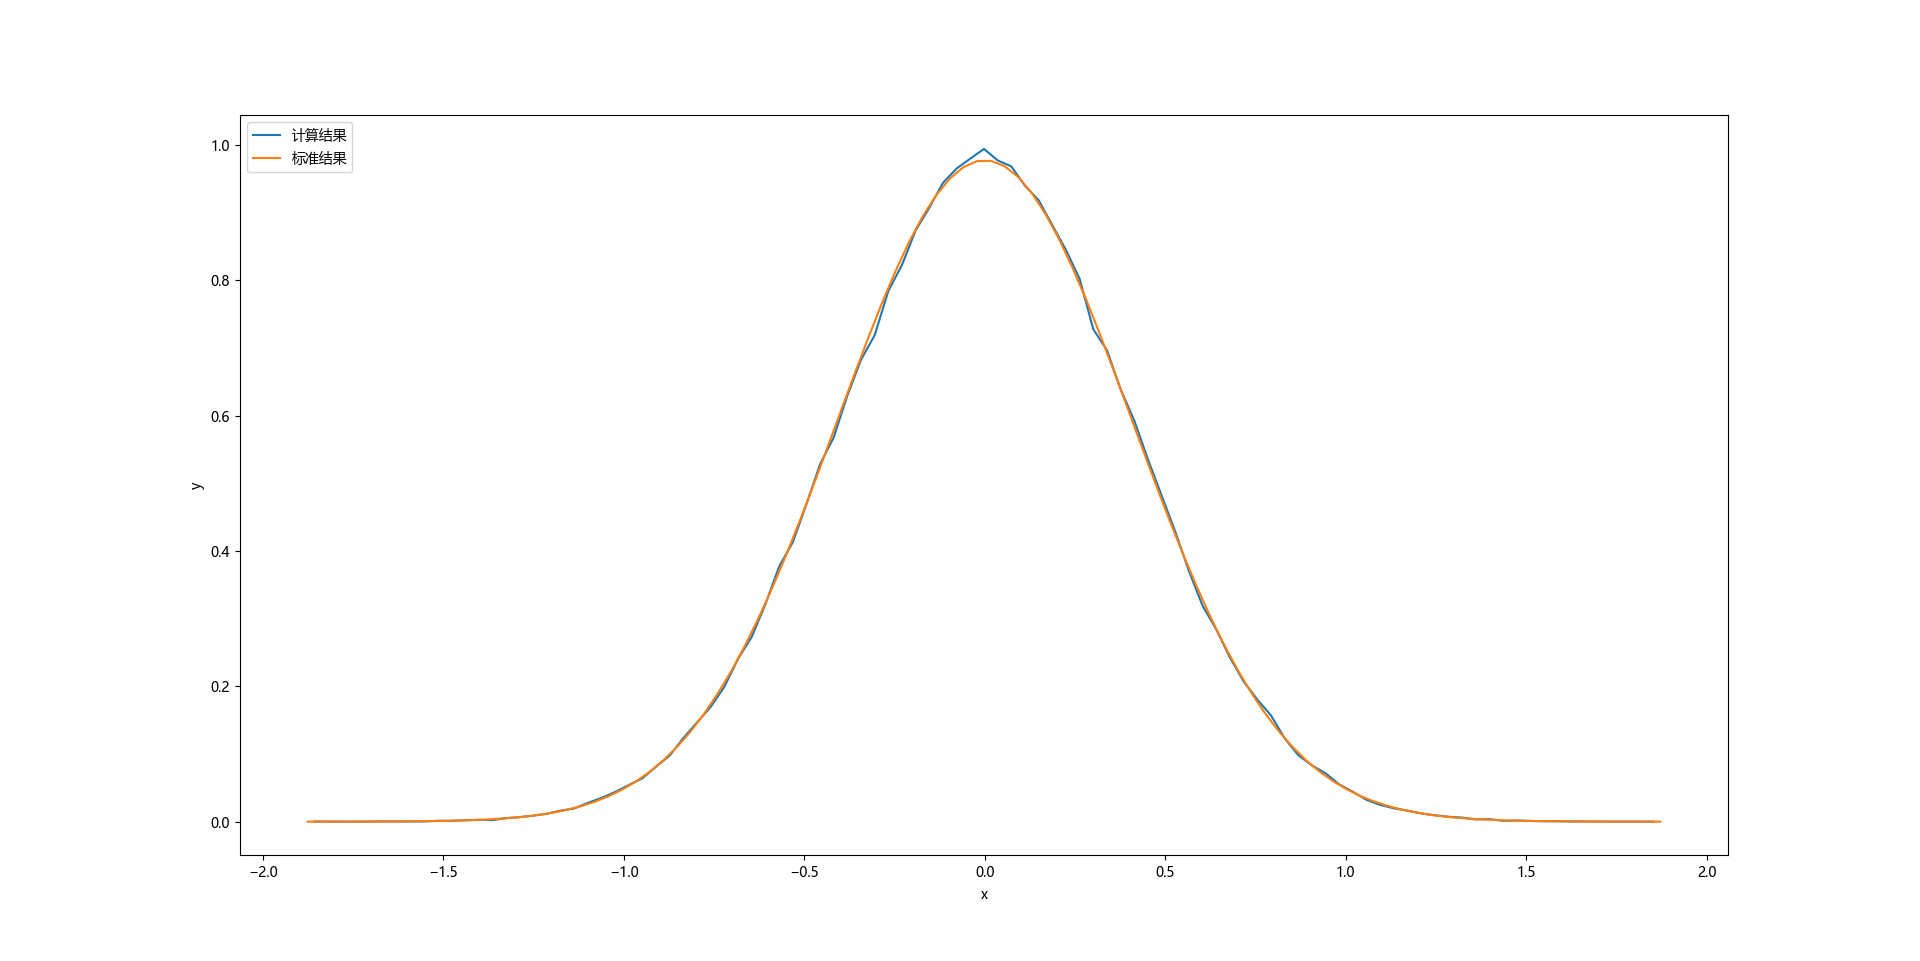
\includegraphics[scale=0.36]{compare}
		\captionsetup{font={small},labelfont=bf}
		\caption{\heiti\zihao{-5}舍选法结果与标准曲线对比图}
		
	\end{figure}
	取$ 10^6 $个随机数点绘图如图1所示,统计结果与原Gaussian曲线基本吻合。
	\begin{figure}[!h]
	
	\centering
	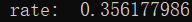
\includegraphics[scale=1]{result_3_6}
	\captionsetup{font={small},labelfont=bf}
	\caption{\heiti\zihao{-5}舍选法抽样效率}
	
\end{figure}


	图2为舍选法抽样效率的输出结果,可见舍选法效率达到0.356以上。
	\section{结论}
所存在的差异主要来源于首先由于结果是统计结果,取点数量不是无穷大,得到的只是频数的相对分布,所以不能和标准曲线完全吻合。其次在统计过程中,由于是连续变量的统计,只能将一定区域划分为小的统计区间逐个区间进行计数,由于实际上概率密度分布应该是对无穷小区间的统计结果,则应该为区间越小,则曲线越平滑,越接近标准曲线。


舍选法的效率与初始设定的a,b,c值有关。c越小,lorentz函数越贴近gauss函数达到相切的位置,在x较大处gauss函数与lorentz函数的比例越大,既F(x)>p(x)允许的情况下b越大a越小,则抽样效率越高。
\end{document}